
%%%%%%%%%%%%%%%%%%%%%%%%%%%%%%%%%%%%%%%%%%%%%%%%%%%%%%%%%%%%%%%%%%%%%%%%%
%       Capítulo 2: Descripción de un robot de 5 grados de libertad     %
%%%%%%%%%%%%%%%%%%%%%%%%%%%%%%%%%%%%%%%%%%%%%%%%%%%%%%%%%%%%%%%%%%%%%%%%%

\chapter{\textcolor{Azul}{Descripción de un robot de 5 grados de libertad}}

\section{Articulaciones y pares cinemáticos}

La movilidad de un sistema puede expresarse en función de los parámetros independientes mínimos que se necesitan para describir de manera única su posición y orientación en un instante de tiempo [6]. Estos parámetros reciben por nombre \textbf{grados de libertad} (GDL). El número de GDL también depende de las dimensiones del espacio en el que se trabaje. Para ejemplificar el caso del movimiento en un espacio plano de dos dimensiones se puede tomar un cuadrado de papel y colocarlo sobre un escritorio, el papel puede moverse de manera vertical (primer GDL), horizontal (segundo GDL) o girar sobre un eje perpendicular al plano (tercer GDL). Dichos movimientos también pueden limitarse. Si ahora se toma un alfiler y se clava el cuadrado de papel sobre el escritorio se han restringido los movimientos horizontales y verticales, quedando únicamente la rotación alrededor del alfiler (solamente un GDL).\\\\En el caso del movimiento plano, los cuerpos rígidos sin restricción cuentan con tres GDL, dos que indican posición y uno que indica orientación. Si se considera ahora el espacio tridimensional, los cuerpos rígidos cuentan con seis GDL, se necesitan tres para definir la posición y otros tres que definen la orientación. \\

\\Los eslabones que componen a un robot manipulador están conectados de tal manera que se permita cierto tipo de movimiento. Existen dos movimientos a partir de los cuales se derivan cualquier movimiento complejo conocido: la traslación pura y la rotación pura. Estas conexiones entre eslabones reciben el nombre de articulaciones o pares cinemáticos [7], Fig \ref{pares}.

\begin{figure}
	\centering
	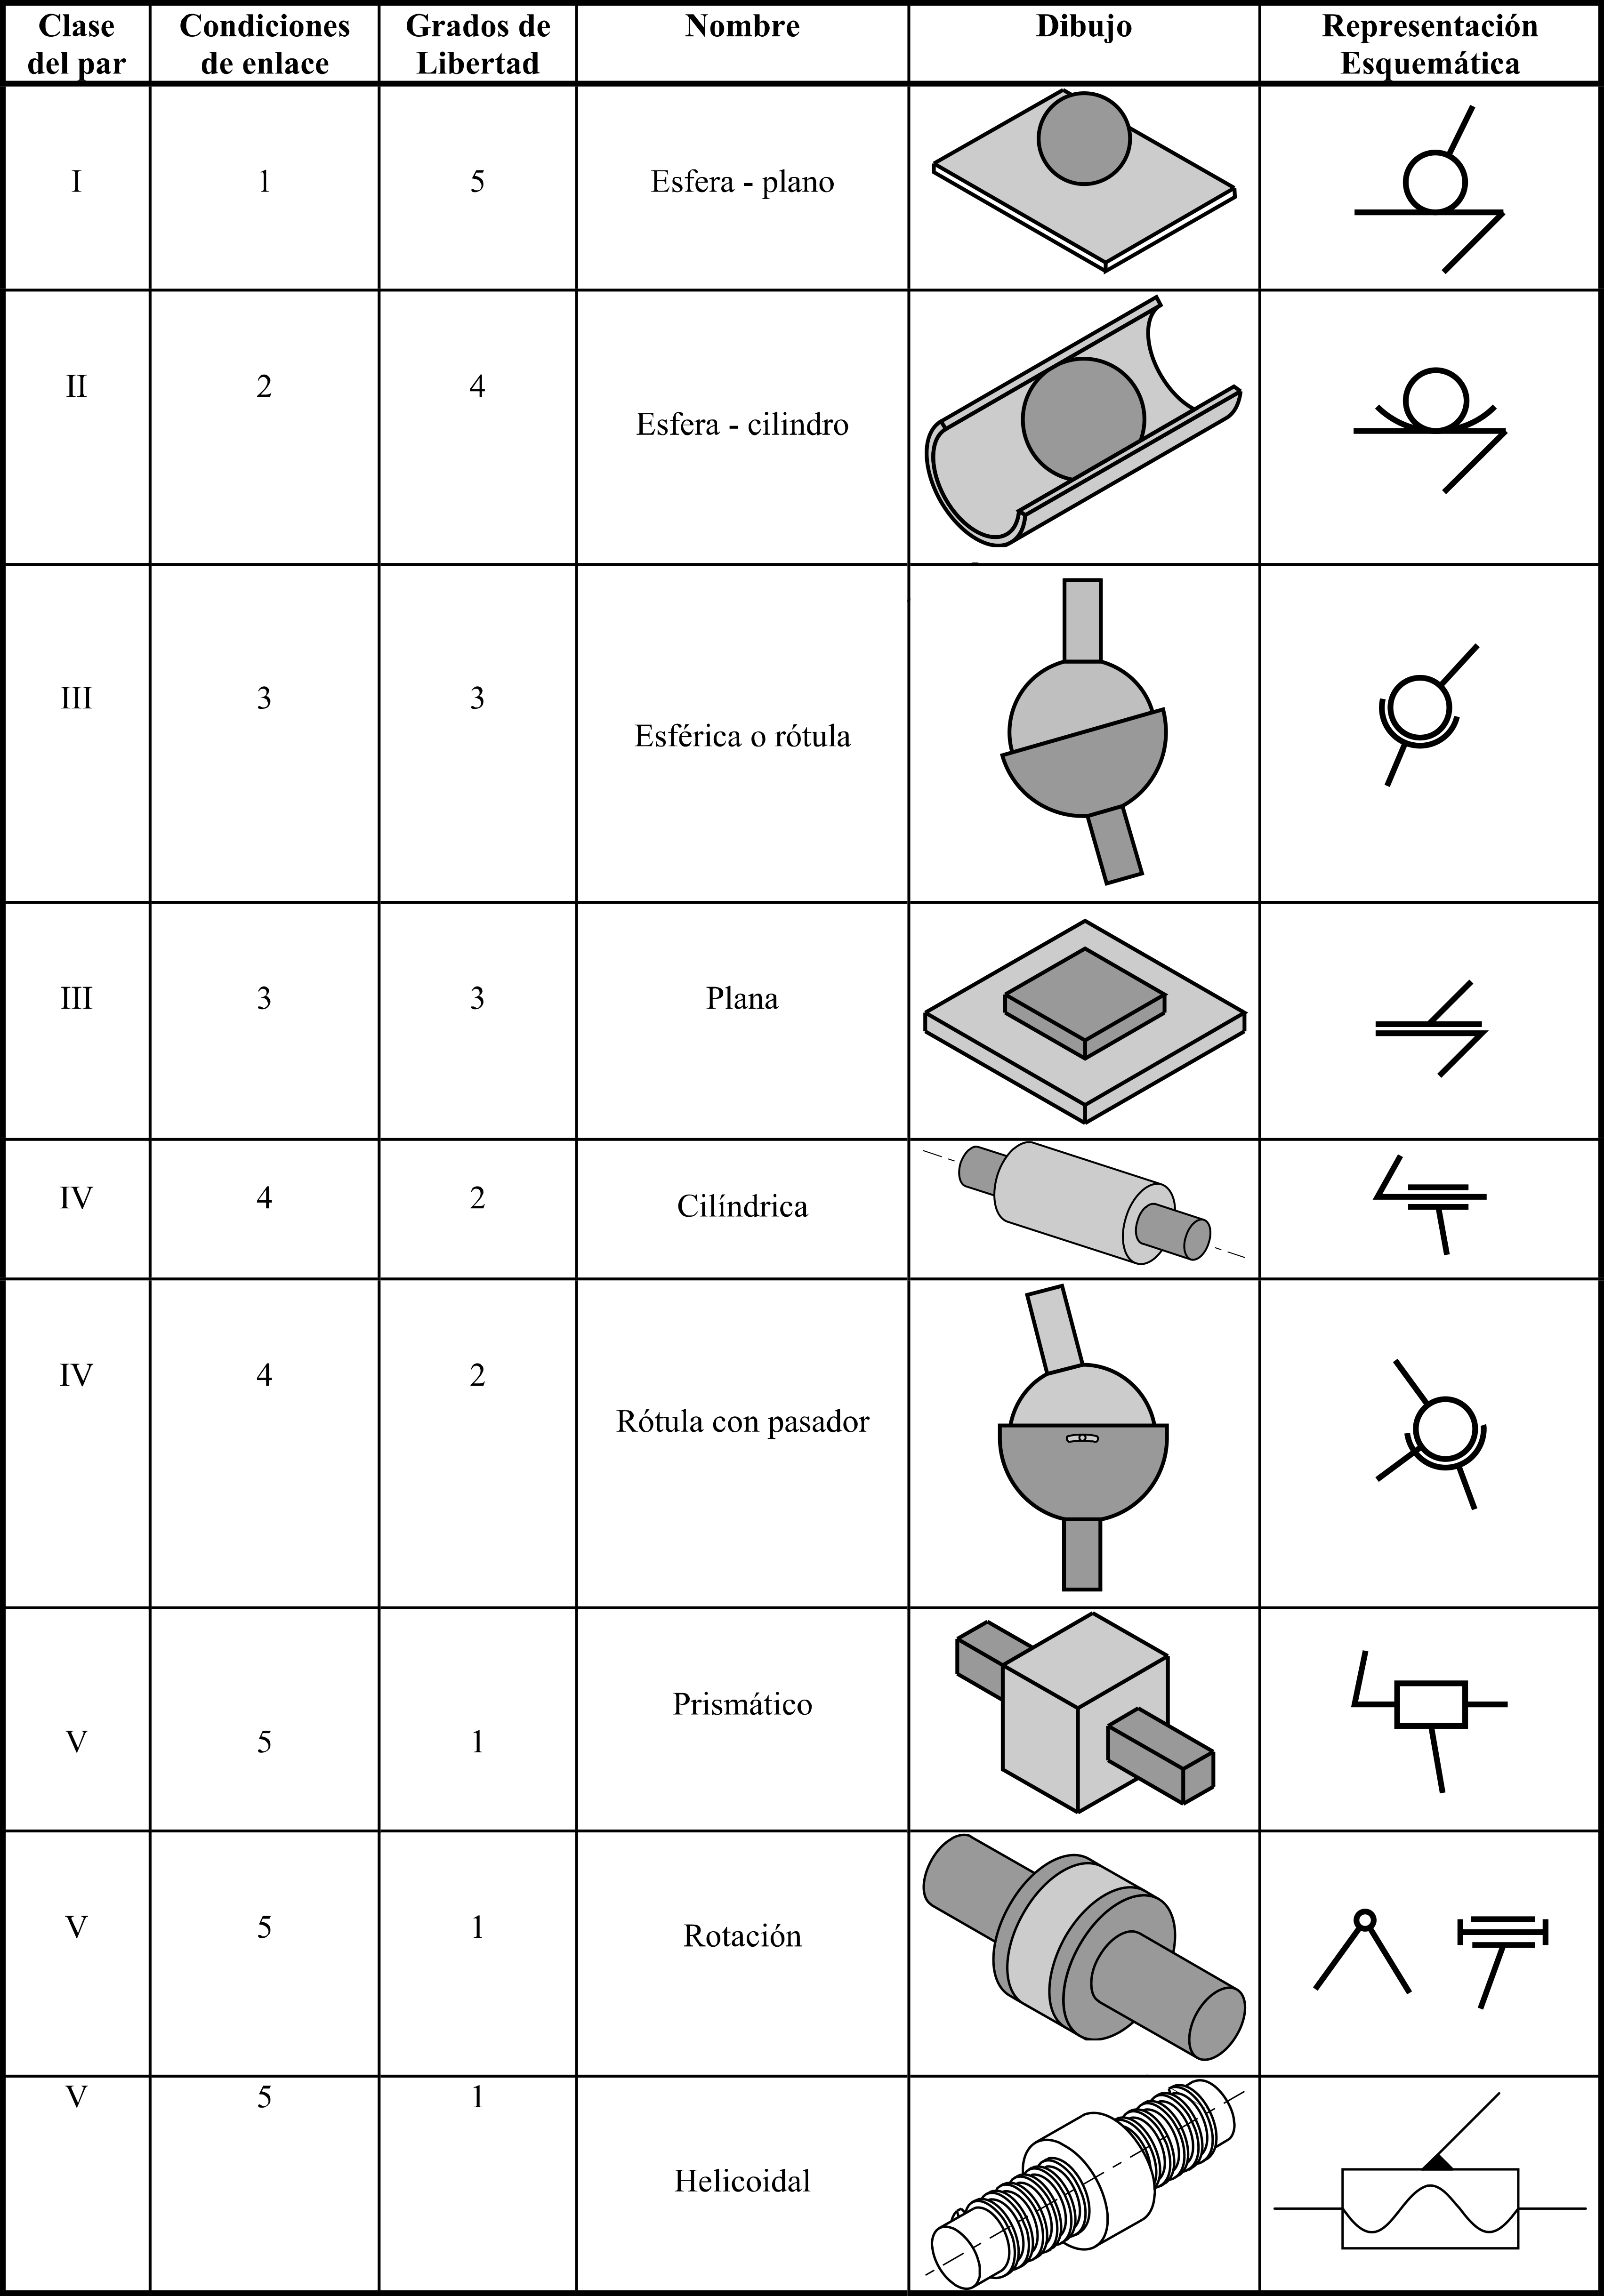
\includegraphics[scale=1.0]{Capitulo2/figs/pares.png} 
	\caption{Pares cinemáticos superiores e inferiores}
	\label{pares}
\end{figure}

\section{Cinemática directa}

Los robots rígidos guardan una relación entre la posición individual de cada articulación y la ubicación espacial de la herramienta o efector final. La cinemática directa consiste en determinar la posición y orientación del efector final con respecto a un sistema de coordenadas que se toma como referencia, conocidos los valores de posición y orientación de las articulaciones y las características geométricas de los elementos del robot. Una parte de la cinemática de los robots se encarga de establecer sistemas de coordenadas para cada eslabón rígido, indicando la posición y orientación respecto a un sistema de referencia inercial, que se relacionan entre sí mediante matrices de transformación. Las operaciones básicas entre sistemas de coordenadas son la traslación y la rotación, que pueden combinarse para obtener matrices de transformaciones homogéneas, como se describirá más adelante.

\subsection{Posición}

En robótica, las instrucciones asignadas a un robot manipulador suelen estar definidas en un espacio de coordenadas cartesianas. Para la asignación de estas coordenadas es necesario un sistema de referencia, como se observa en la figura \ref{sistemasdereferencia}, donde las coordenadas del punto $p$ pueden ser descritas con referencia al sistema $o_{0}x_{0}y_{0}$ o al sistema $o_{1}x_{1}y_{1}$.
\begin{figure}[h!]
	\centering
	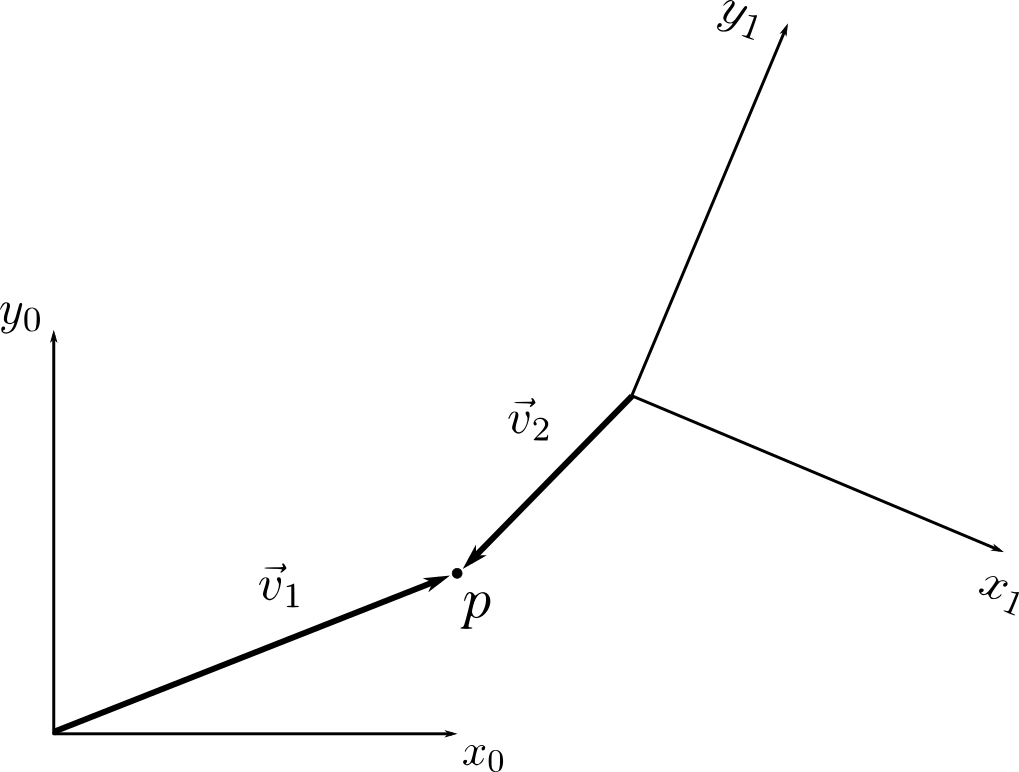
\includegraphics[scale=0.3]{Capitulo2/figs/SistemaPuntoVectores.png} 
	\caption{Dos sistemas de referencia, un punto p y dos vectores $\vec{v}_{1}$ y $\vec{v}_{2}$.}
	\label{sistemasdereferencia}
\end{figure}
\\\\Para que la notación sea clara, al hacer referencia a uno u otro sistema se colocará un superíndice que indique el sistema utilizado. De esta manera, de acuerdo a la fig \ref{sistemasdereferencia} podemos asignar al punto $p$ el valor $(a,b)^T$ correspondiente al sistema $o_{0}x_{0}y_{0}$  o el valor $(c,d)^T$ correspondiente al sistema $o_{1}x_{1}y_{1}$, esto es
\[
p^{0}=
\begin{bmatrix} 
a  \\
b
\end{bmatrix}
,\quad
p^{1}=
\begin{bmatrix} 
c  \\
d
\end{bmatrix}
\]

Es importante recordar que $p$ es una representación del punto como entidad geométrica, mientras que $p_{0}$ y $p_{1}$ son vectores de coordenadas que representan la localización que $p$ en el espacio, por lo tanto $p\neq p^{0}$ y $p\neq p^{1}$.\\\\
Dado que el origen de un sistema de coordenadas es la representación de un punto en el espacio, es posible escribir a los vectores de coordenadas que representan la posición del origen de un sistema con respecto al otro. En la figura \ref{sistemasdereferencia} por ejemplo
\[
O_1^0 = 
\begin{bmatrix}
e\\
f
\end{bmatrix}
,\quad
O_0^1 = 
\begin{bmatrix}
-g\\
-h
\end{bmatrix}
\]

En el caso de un solo sistema de coordenadas no se colocará el superíndice en la notación. Es importante notar la diferencia entre el punto $p$ como entidad geométrica y el vector de coordenadas que se usa para representar a $p$. Mientras que el punto $p$ corresponde a una ubicación específica en el espacio, el vector de coordenadas representa una dirección y una magnitud, por lo que no está fijo en el espacio y depende del sistema de referencia.

%%%%%%%%$\vec{o}^{\,t}

\subsection{Orientación}



\section{Cinemática inversa}

\section{Modelado}

%inserción de codigo de Matlab
%Es conveniente sangrarlo (los de proteco dicen "indentarlo") para que no se encime con los números de las líneas a la izquierda
\begin{lstlisting}[frame=single]
    % Declaracion de las variables simbolicas
\end{lstlisting}